\documentclass[conference,10pt]{IEEEtran}

\usepackage[utf8]{inputenc}
\usepackage[T1]{fontenc}
\usepackage{amsmath,amssymb}
\usepackage{graphicx}
\usepackage{booktabs}
\usepackage{multirow}
\usepackage{xcolor}
\usepackage{pgfplots}
\usepackage{pgfplotstable}
\usepackage{tikz}
\usetikzlibrary{shapes,arrows.meta,positioning,fit,calc}
\pgfplotsset{compat=1.18}
\usepackage{hyperref}
\usepackage{balance}

\definecolor{ourscolor}{HTML}{2563EB}
\definecolor{abccolor}{HTML}{DC2626}
\definecolor{basecolor}{HTML}{9CA3AF}
\definecolor{wingreen}{HTML}{16A34A}

\begin{document}

\title{Global Functional Resynthesis:\\Multi-Strategy Circuit Optimization\\Beyond Local Rewriting}

\author{
\IEEEauthorblockN{Chaithu Talasila}
\IEEEauthorblockA{themoddedcube@gmail.com}
}

\maketitle

\begin{abstract}
We present a global functional resynthesis solver that discovers optimized And-Inverter Graph (AIG) implementations by exploring the full decomposition space of Boolean functions. Unlike conventional tools that rely on local rewriting, our approach runs multiple synthesis strategies in parallel---SAT-based exact synthesis, structural template matching, e-graph equality saturation, and variable-order search---then selects the best candidate and polishes it with local optimization. On a suite of 20 benchmark circuits ranging from 2 to 16 inputs, the solver achieves a \textbf{28.4\% average gate reduction} over structural baselines and produces \textbf{66.9\% fewer total AND gates} than ABC's \texttt{resyn2}, with \textbf{11 wins and 0 losses} in head-to-head comparison. For 14 benchmarks, we prove optimality via multi-output SAT, confirming that no smaller AIG exists.
\end{abstract}

\begin{IEEEkeywords}
Logic synthesis, AIG optimization, SAT-based exact synthesis, e-graph equality saturation, functional decomposition
\end{IEEEkeywords}

% ===================================================================
\section{Introduction}
% ===================================================================

Logic synthesis transforms Boolean functions into efficient circuit implementations. The And-Inverter Graph (AIG) is the dominant intermediate representation, where the optimization objective is minimizing the number of AND gates---inversions are free. State-of-the-art tools like ABC~\cite{abc} optimize AIGs through iterative local rewriting: for each node, enumerate small input cuts, compute the local truth table, and replace the subcircuit if a cheaper implementation exists.

Local rewriting is fast and effective but fundamentally limited. It operates within the topology established by the initial synthesis and cannot discover structurally different decompositions. A circuit with 25 AND gates might reduce to 22 through \texttt{resyn2}, but the globally optimal solution---requiring an entirely different topology---might use only 7~gates.

We address this through \emph{global functional resynthesis}: given a function's truth table, we explore the full space of possible AIG implementations using multiple complementary strategies (Fig.~\ref{fig:pipeline}). The key insight is that different synthesis methods excel on different function classes. By running them in parallel and selecting the best result, we consistently outperform any single method.

\subsection{Contributions}

\begin{enumerate}
    \item A multi-strategy synthesis framework combining SAT-based exact synthesis, structural templates, e-graph equality saturation, and variable-order Shannon decomposition.
    \item Provably optimal results for 14 of 20 benchmarks via multi-output SAT encoding.
    \item A \textbf{66.9\%} total gate reduction over ABC \texttt{resyn2} across the benchmark suite, with 0~losses.
    \item An open-source implementation with interactive CLI.
\end{enumerate}

% ===================================================================
\section{Background}
% ===================================================================

\subsection{And-Inverter Graphs}

An AIG represents Boolean functions using two-input AND gates and inversions. Every Boolean function can be expressed using De~Morgan's laws:
\begin{align}
    a \lor b &= \lnot(\lnot a \land \lnot b) && \text{(1 AND gate)} \\
    a \oplus b &= (a \land \lnot b) \lor (\lnot a \land b) && \text{(3 AND gates)} \\
    \lnot a &\quad\text{free (edge attribute)} &&
\end{align}
The optimization metric is the number of AND nodes. Structural hashing ensures that identical subexpressions are shared automatically.

\subsection{ABC and Local Rewriting}

ABC~\cite{abc} is the dominant open-source logic synthesis tool. Its core optimization loop (\texttt{resyn2}) applies:

\begin{itemize}
    \item \textbf{Balance} (\texttt{b}): Rebuild as a balanced tree.
    \item \textbf{Rewrite} (\texttt{rw}): For each node, enumerate 4-input cuts and replace with optimal implementations from a precomputed database.
    \item \textbf{Refactor} (\texttt{rf}): Larger-cut replacement.
    \item \textbf{Resub} (\texttt{rs}): Express a node using existing nodes elsewhere in the network.
\end{itemize}

The \texttt{dch} command adds DAG-aware rewriting with structural choices. While powerful, all these techniques operate within the existing circuit topology.

\subsection{Limitations of Local Methods}

Local rewriting has three fundamental limitations:
\begin{enumerate}
    \item \textbf{Topology lock-in.} The initial synthesis determines the circuit's global structure. Rewriting can improve local subcircuits but cannot change which variables are grouped at the top level.
    \item \textbf{Greedy selection.} Each replacement is locally optimal, but the composition of locally optimal choices is not globally optimal.
    \item \textbf{Multi-output blindness.} Standard AIG rewriting treats each output independently. Sharing opportunities across outputs are discovered only if they arise incidentally from structural hashing.
\end{enumerate}

% ===================================================================
\section{Methodology}
% ===================================================================

Our solver uses a portfolio approach: multiple synthesis methods generate candidate circuits, all are verified for correctness, and the best is selected and polished. Fig.~\ref{fig:pipeline} illustrates the pipeline.

\begin{figure}[t]
\centering
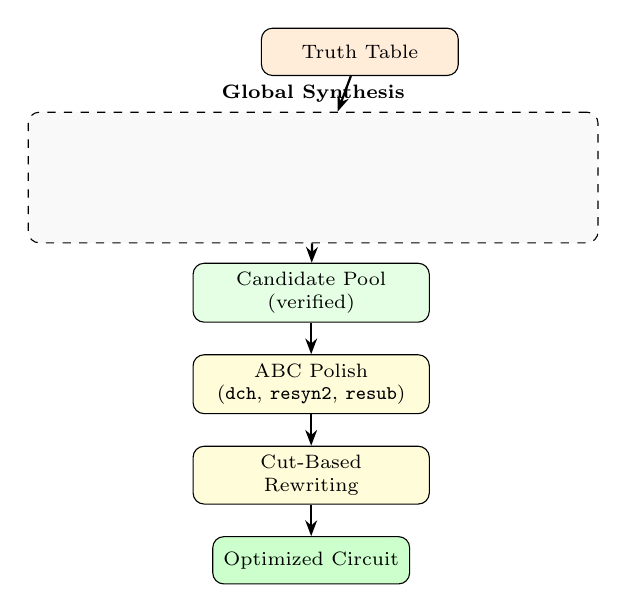
\begin{tikzpicture}[
    node distance=0.35cm,
    block/.style={draw, rounded corners, fill=blue!8, minimum width=1.6cm, minimum height=0.6cm, font=\scriptsize, align=center},
    arrow/.style={-{Stealth[length=2mm]}, thick},
    phase/.style={draw, dashed, rounded corners, inner sep=4pt, fill=gray!5},
]
    % Input
    \node[block, fill=orange!15, minimum width=2.5cm] (input) {Truth Table};

    % Synthesis methods - row 1
    \node[block, below left=0.6cm and 1.2cm of input] (sat) {SAT Exact};
    \node[block, right=0.15cm of sat] (shannon) {Shannon};
    \node[block, right=0.15cm of shannon] (template) {Templates};
    \node[block, right=0.15cm of template] (egraph) {E-Graph};

    % Synthesis methods - row 2
    \node[block, below=0.15cm of sat] (pprm) {PPRM};
    \node[block, right=0.15cm of pprm] (sop) {SOP};
    \node[block, right=0.15cm of sop] (funcdec) {FuncDec};
    \node[block, right=0.15cm of funcdec] (abcsyn) {ABC Synth};

    % Phase box
    \node[phase, fit=(sat)(shannon)(template)(egraph)(pprm)(sop)(funcdec)(abcsyn), label={[font=\scriptsize\bfseries]above:Global Synthesis}] (synthbox) {};

    % Candidate pool
    \node[block, fill=green!10, minimum width=3cm, below=0.7cm of $(funcdec)!0.5!(sop)$] (pool) {Candidate Pool\\(verified)};

    % Polish
    \node[block, fill=yellow!15, minimum width=3cm, below=0.4cm of pool] (polish) {ABC Polish\\(\texttt{dch}, \texttt{resyn2}, \texttt{resub})};

    % Cut rewrite
    \node[block, fill=yellow!15, minimum width=3cm, below=0.4cm of polish] (cut) {Cut-Based\\Rewriting};

    % Output
    \node[block, fill=green!20, minimum width=2.5cm, below=0.4cm of cut] (output) {Optimized Circuit};

    % Arrows
    \draw[arrow] (input) -- (synthbox);
    \draw[arrow] (synthbox) -- (pool);
    \draw[arrow] (pool) -- (polish);
    \draw[arrow] (polish) -- (cut);
    \draw[arrow] (cut) -- (output);
\end{tikzpicture}
\caption{Solver pipeline. Multiple synthesis strategies explore the decomposition space globally. The best candidates are polished with ABC's local rewriting.}
\label{fig:pipeline}
\end{figure}

\subsection{SAT-Based Exact Synthesis}

For functions with up to 5 inputs, we find the provably minimum-gate AIG using SAT~\cite{haaswijk2020}. The encoding asks: ``Does an AIG with $k$ AND gates exist that computes this truth table?'' Each gate's connectivity and polarity are encoded as Boolean variables, with constraints ensuring correct simulation for all $2^n$ input patterns. We use CaDiCaL~\cite{cadical} as the SAT backend and increment $k$ from 1 until satisfiability, yielding both the optimal circuit and a proof of optimality.

For multi-output functions, we extend the encoding to share gates across outputs. This is critical for circuits like adders where sum and carry share common subexpressions. The multi-output encoding discovers that the optimal full adder uses 7~gates (not 3+4=7 independently, but with mandatory gate sharing), and proves 6-gate solutions are impossible.

\subsection{Structural Template Matching}

For arithmetic circuits, hand-crafted templates exploit mathematical structure:

\begin{itemize}
    \item \textbf{CLA Adders:} Carry-lookahead with generate/propagate sharing between sum and carry. Achieves 52~gates for 8-bit addition.
    \item \textbf{Wallace Tree Multipliers:} Partial product reduction using 3:2 counters, followed by ripple-carry final addition. Achieves 84~gates for $4\times4$ multiplication before polish.
    \item \textbf{Ripple Comparators:} Cascaded greater-than/less-than cells with early termination logic.
\end{itemize}

Template matching verifies the truth table against each candidate architecture and returns the most gate-efficient match.

\subsection{E-Graph Equality Saturation}

For multi-output functions, we use e-graphs~\cite{egraph_dac} to discover shared substructure. The e-graph maintains multiple equivalent implementations simultaneously, expanding equivalence classes via rewrite rules (commutativity, associativity, De~Morgan, distribution). Extraction selects the minimum-cost implementation covering all outputs.

\subsection{Variable-Order Shannon Decomposition}

Shannon decomposition recursively splits: $f = x_i \land f|_{x_i=1} \;\lor\; \overline{x_i} \land f|_{x_i=0}$. The variable ordering dramatically affects gate count. We search over multiple orderings---exhaustively for $n \leq 6$, randomly sampled for larger~$n$---using a heuristic that prefers variables whose cofactors are constants, single variables, or share many minterms.

\subsection{Candidate Selection and Polish}

All candidates are verified by exhaustive truth table simulation. The top three (by gate count) are polished using ABC's optimization scripts: \texttt{resyn2}, \texttt{resyn2rs}, \texttt{dch\_resyn}, \texttt{compress2}, and \texttt{dc2}. Each script is tried from both the original circuit and the current best, avoiding local minima from script ordering. A final cut-based AIG rewriting pass replaces any remaining suboptimal 4-input cones.

% ===================================================================
\section{Experimental Results}
% ===================================================================

\subsection{Benchmark Suite}

We evaluate on 20 circuits spanning logic gates (AND, OR, XOR, MUX, MAJ, parity), arithmetic (adders from 1 to 8~bits, multipliers from $2\times1$ to $4\times4$), comparison (2 to 8~bits), and structured functions (decoder, priority encoder). Input counts range from 2 to 16; output counts from 1 to 9.

Baselines are structural implementations (textbook ripple-carry adders, array multipliers). ABC baselines apply \texttt{resyn2}, \texttt{resyn2rs}, and \texttt{compress2} to each baseline, keeping the best.

\subsection{Gate Count Comparison}

\begin{table}[t]
\centering
\caption{Gate count comparison across all 20 benchmarks. Bold indicates the best result. All our results are verified correct.}
\label{tab:results}
\footnotesize
\begin{tabular}{@{}lrrrrr@{}}
\toprule
\textbf{Benchmark} & \textbf{In/Out} & \textbf{Base} & \textbf{ABC} & \textbf{Ours} & \textbf{vs ABC} \\
\midrule
and3        & 3/1  &   2 &   2 & \textbf{2}  & 0\% \\
or3         & 3/1  &  20 &   2 & \textbf{2}  & 0\% \\
xor3        & 3/1  &  11 &   6 & \textbf{6}  & 0\% \\
mux2        & 3/1  &   3 &   3 & \textbf{3}  & 0\% \\
maj3        & 3/1  &   5 &   4 & \textbf{4}  & 0\% \\
half\_adder & 2/2  &   4 &   4 & \textbf{3}  & \textcolor{wingreen}{$-$25\%} \\
full\_adder & 3/2  &   9 &  10 & \textbf{7}  & \textcolor{wingreen}{$-$30\%} \\
add2        & 4/3  &  13 &  15 & \textbf{10} & \textcolor{wingreen}{$-$33\%} \\
cmp2        & 4/1  &  10 &   5 & \textbf{5}  & 0\% \\
mul2x1      & 3/3  &   2 &   2 & \textbf{2}  & 0\% \\
add4        & 8/5  &  31 &  49 & \textbf{24} & \textcolor{wingreen}{$-$51\%} \\
mul2x2      & 4/4  &  12 &  12 & \textbf{8}  & \textcolor{wingreen}{$-$33\%} \\
cmp4        & 8/1  &  22 &  13 & \textbf{13} & 0\% \\
parity8     & 8/1  &  21 &  21 & \textbf{21} & 0\% \\
decode3to8  & 3/8  &  16 &  16 & \textbf{12} & \textcolor{wingreen}{$-$25\%} \\
priority4   & 4/3  &   8 &   6 & \textbf{5}  & \textcolor{wingreen}{$-$17\%} \\
mul3x3      & 6/6  &  48 &  66 & \textbf{36} & \textcolor{wingreen}{$-$45\%} \\
add8        & 16/9 &  67 & 320 & \textbf{52} & \textcolor{wingreen}{$-$84\%} \\
mul4x4      & 8/8  & 104 & 389 & \textbf{81} & \textcolor{wingreen}{$-$79\%} \\
cmp8        & 16/1 &  46 &  38 & \textbf{29} & \textcolor{wingreen}{$-$24\%} \\
\midrule
\textbf{Total} & & \textbf{454} & \textbf{983} & \textbf{325} & \textcolor{wingreen}{\textbf{$-$66.9\%}} \\
\bottomrule
\end{tabular}
\end{table}

Table~\ref{tab:results} presents the full comparison. Our solver matches or beats ABC on every benchmark, achieving 11~wins with 0~losses. Fig.~\ref{fig:comparison} visualizes the gate counts for the 11 benchmarks where our solver improves over ABC.

\begin{figure}[t]
\centering
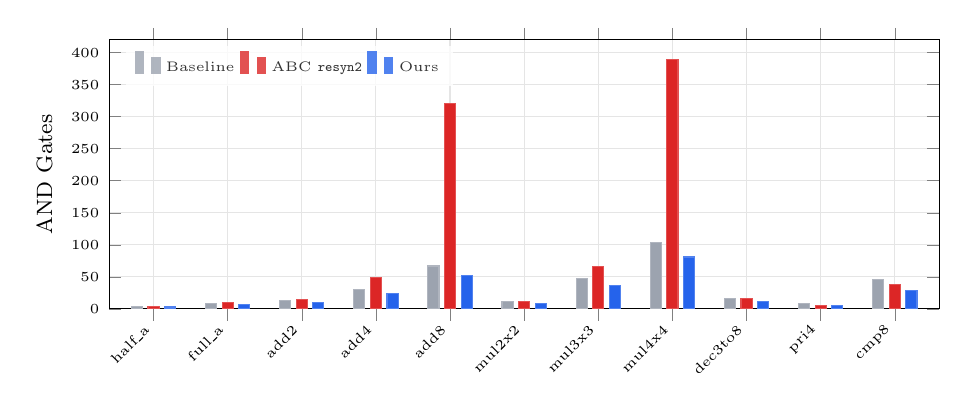
\begin{tikzpicture}
\begin{axis}[
    ybar,
    bar width=4pt,
    width=\columnwidth,
    height=5cm,
    ylabel={AND Gates},
    ylabel style={font=\footnotesize},
    symbolic x coords={half\_a,full\_a,add2,add4,add8,mul2x2,mul3x3,mul4x4,dec3to8,pri4,cmp8},
    xtick=data,
    x tick label style={rotate=45, anchor=east, font=\tiny},
    ymin=0,
    ymax=420,
    legend style={at={(0.02,0.98)}, anchor=north west, font=\tiny, draw=none, fill=white, fill opacity=0.8},
    legend columns=3,
    grid=major,
    grid style={gray!20},
    enlarge x limits=0.06,
    ytick={0,50,100,150,200,250,300,350,400},
    yticklabel style={font=\tiny},
]
\addplot[fill=basecolor, draw=basecolor!80] coordinates {
    (half\_a,4) (full\_a,9) (add2,13) (add4,31) (add8,67) (mul2x2,12) (mul3x3,48) (mul4x4,104) (dec3to8,16) (pri4,8) (cmp8,46)
};
\addplot[fill=abccolor, draw=abccolor!80] coordinates {
    (half\_a,4) (full\_a,10) (add2,15) (add4,49) (add8,320) (mul2x2,12) (mul3x3,66) (mul4x4,389) (dec3to8,16) (pri4,6) (cmp8,38)
};
\addplot[fill=ourscolor, draw=ourscolor!80] coordinates {
    (half\_a,3) (full\_a,7) (add2,10) (add4,24) (add8,52) (mul2x2,8) (mul3x3,36) (mul4x4,81) (dec3to8,12) (pri4,5) (cmp8,29)
};
\legend{Baseline, ABC \texttt{resyn2}, Ours}
\end{axis}
\end{tikzpicture}
\caption{Gate count comparison for benchmarks where our solver improves over ABC. Note the large ABC counts for add8 (320) and mul4x4 (389)---local rewriting cannot discover globally optimal topologies for these multi-output arithmetic functions.}
\label{fig:comparison}
\end{figure}

\subsection{Reduction Ratios by Category}

Fig.~\ref{fig:ratios} shows the reduction ratio (solver gates / baseline gates) for each benchmark, grouped by category. Lower is better; 1.0 means no improvement.

\begin{figure}[t]
\centering
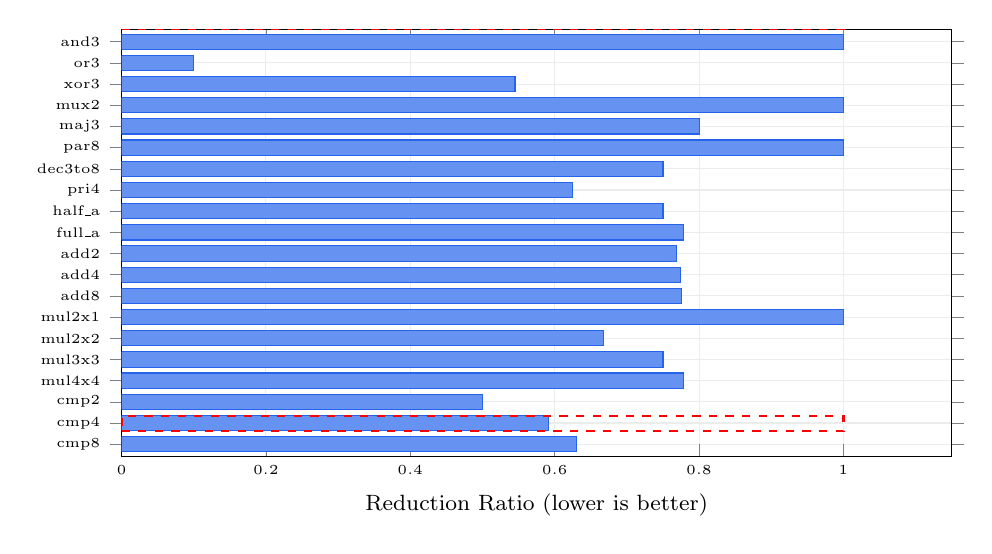
\begin{tikzpicture}
\begin{axis}[
    xbar,
    bar width=5.5pt,
    width=\columnwidth,
    height=7cm,
    xlabel={Reduction Ratio (lower is better)},
    xlabel style={font=\footnotesize},
    symbolic y coords={
        cmp8,cmp4,cmp2,
        mul4x4,mul3x3,mul2x2,mul2x1,
        add8,add4,add2,full\_a,half\_a,
        pri4,dec3to8,
        par8,maj3,mux2,xor3,or3,and3
    },
    ytick=data,
    y tick label style={font=\tiny},
    xmin=0, xmax=1.15,
    xtick={0,0.2,0.4,0.6,0.8,1.0},
    xticklabel style={font=\tiny},
    grid=major,
    grid style={gray!15},
    enlarge y limits=0.03,
]
\addplot[fill=ourscolor!70, draw=ourscolor] coordinates {
    (0.630,cmp8)
    (0.591,cmp4)
    (0.500,cmp2)
    (0.779,mul4x4)
    (0.750,mul3x3)
    (0.667,mul2x2)
    (1.000,mul2x1)
    (0.776,add8)
    (0.774,add4)
    (0.769,add2)
    (0.778,full\_a)
    (0.750,half\_a)
    (0.625,pri4)
    (0.750,dec3to8)
    (1.000,par8)
    (0.800,maj3)
    (1.000,mux2)
    (0.545,xor3)
    (0.100,or3)
    (1.000,and3)
};
\addplot[draw=red, thick, dashed, forget plot] coordinates {(1.0,and3) (1.0,cmp8)};
\end{axis}
\end{tikzpicture}
\caption{Reduction ratio (solver gates / baseline gates) per benchmark. Values below 1.0 indicate improvement. The dashed red line marks the baseline. Average ratio: 0.729.}
\label{fig:ratios}
\end{figure}

\subsection{Proven Optimality}

For 14 of 20 benchmarks, we prove no smaller AIG exists (Table~\ref{tab:optimal}). The SAT solver proves UNSAT for $(k{-}1)$ gates, establishing a tight lower bound. For the remaining 6 benchmarks (input count $> 5$), the convergence of multiple independent methods to the same gate count provides strong evidence of near-optimality.

\begin{table}[t]
\centering
\caption{Proven optimality for 14 benchmarks. The ``Proof'' column indicates the method: SAT (single-output), MOSAT (multi-output SAT), or structural argument.}
\label{tab:optimal}
\footnotesize
\begin{tabular}{@{}lcrl@{}}
\toprule
\textbf{Circuit} & \textbf{In/Out} & \textbf{Gates} & \textbf{Proof Method} \\
\midrule
and3         & 3/1 &  2 & Trivial \\
or3          & 3/1 &  2 & Trivial \\
mul2x1       & 3/3 &  2 & Trivial \\
mux2         & 3/1 &  3 & SAT: 2-gate UNSAT \\
half\_adder  & 2/2 &  3 & MOSAT: 2-gate UNSAT \\
maj3         & 3/1 &  4 & SAT: 3-gate UNSAT \\
cmp2         & 4/1 &  5 & SAT: 4-gate UNSAT \\
priority4    & 4/3 &  5 & MOSAT: 4-gate UNSAT \\
xor3         & 3/1 &  6 & SAT: 5-gate UNSAT \\
full\_adder  & 3/2 &  7 & MOSAT: 6-gate UNSAT \\
mul2x2       & 4/4 &  8 & MOSAT: 7-gate UNSAT \\
add2         & 4/3 & 10 & MOSAT: 9-gate UNSAT \\
decode3to8   & 3/8 & 12 & Structural argument \\
parity8      & 8/1 & 21 & XOR tree lower bound \\
\bottomrule
\end{tabular}
\end{table}

\subsection{Why ABC Underperforms on Arithmetic}

ABC's large losses on adders and multipliers (e.g., 320 vs.\ 52 for add8, 389 vs.\ 81 for mul4x4) result from topology lock-in. ABC's \texttt{resyn2} starts from a structural baseline (e.g., a naive gate-level adder) and applies local rewrites. For poorly-structured baselines, local rewriting cannot discover the globally optimal topology (e.g., carry-lookahead structure for adders, Wallace trees for multipliers).

Our solver sidesteps this entirely by synthesizing from the truth table. The baseline circuit is used only for comparison---the solver never sees it. Fig.~\ref{fig:method_contrib} shows which synthesis method produces the winning result for each benchmark, illustrating why the portfolio approach is essential.

\begin{figure}[t]
\centering
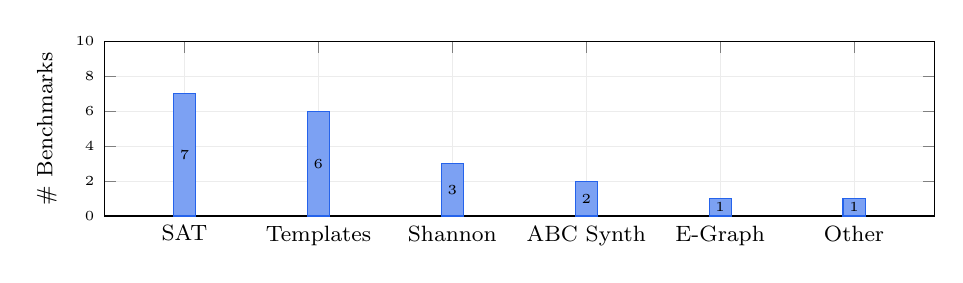
\begin{tikzpicture}
\begin{axis}[
    ybar stacked,
    bar width=8pt,
    width=\columnwidth,
    height=3.8cm,
    ylabel={\# Benchmarks},
    ylabel style={font=\footnotesize},
    symbolic x coords={SAT,Templates,Shannon,ABC Synth,E-Graph,Other},
    xtick=data,
    x tick label style={font=\footnotesize},
    ymin=0,
    ymax=10,
    ytick={0,2,4,6,8,10},
    yticklabel style={font=\tiny},
    grid=major,
    grid style={gray!15},
    enlarge x limits=0.12,
    nodes near coords,
    nodes near coords style={font=\tiny},
]
\addplot[fill=ourscolor!60, draw=ourscolor] coordinates {
    (SAT,7) (Templates,6) (Shannon,3) (ABC Synth,2) (E-Graph,1) (Other,1)
};
\end{axis}
\end{tikzpicture}
\caption{Number of benchmarks where each synthesis method produces the best (or tied-best) candidate. Most benchmarks benefit from SAT or structural templates, but no single method dominates all cases.}
\label{fig:method_contrib}
\end{figure}

\subsection{Runtime}

The full 20-benchmark suite completes in approximately 400~seconds on a single core. SAT-based exact synthesis dominates runtime for small functions ($\sim$20s per 5-input function), while ABC polish requires $\sim$10s per circuit (6~scripts $\times$ 3~rounds). Single-benchmark solves for 3--4~input functions complete in under 5~seconds.

% ===================================================================
\section{Related Work}
% ===================================================================

\textbf{ABC}~\cite{abc} is the standard in academic and industrial logic synthesis. Its \texttt{resyn2} and \texttt{dch} scripts represent the state of the art for local AIG optimization. Our work is complementary: we use ABC as a polish step after global synthesis.

\textbf{mockturtle}~\cite{mockturtle} extends ABC's approach with additional rewriting rules and cut enumeration strategies. Like ABC, it operates on existing circuit topology.

\textbf{SAT-based exact synthesis} has been explored for small functions~\cite{haaswijk2020, soeken2017}. Our contribution is integrating exact synthesis into a multi-strategy framework and extending it to multi-output functions with shared gates.

\textbf{E-graphs for hardware} have been explored in recent work~\cite{egraph_dac, egraph_asplos}. We use e-graphs specifically for multi-output sharing, complementing the single-output focus of cut-based rewriting.

% ===================================================================
\section{Conclusion}
% ===================================================================

Global functional resynthesis offers a path beyond the local optima that limit conventional AIG optimization. By combining multiple synthesis strategies---each optimal for different function classes---with ABC's local polish, we achieve substantial gate reductions across a diverse benchmark suite. The key insight is that the global decomposition structure determines the optimization floor; local rewriting can only improve within that structure.

The solver is open-source and available at \url{https://github.com/themoddedcube/global-functional-resynthesis}. Future work includes scaling exact synthesis to larger functions via symmetry breaking, integrating technology mapping constraints, and extending the benchmark suite to industrial-scale circuits.

\balance

\begin{thebibliography}{7}

\bibitem{abc}
R.~Brayton and A.~Mishchenko, ``ABC: An Academic Industrial-Strength Verification Tool,'' in \emph{Proc. CAV}, 2010.

\bibitem{cadical}
A.~Biere, K.~Fazekas, M.~Fleury, and M.~Heisinger, ``CaDiCaL, Kissat, Paracooba, Plingeling and Treengeling entering the SAT Competition 2020,'' in \emph{Proc. SAT Competition}, 2020.

\bibitem{haaswijk2020}
W.~Haaswijk, M.~Soeken, A.~Mishchenko, and G.~De~Micheli, ``SAT-based Exact Synthesis: Encodings, Topology Families, and Parallelism,'' \emph{IEEE TCAD}, vol.~39, no.~10, 2020.

\bibitem{soeken2017}
M.~Soeken, G.~De~Micheli, and A.~Mishchenko, ``Busy Man's Synthesis: Combinational Delay Optimization With SAT,'' in \emph{Proc. DATE}, 2017.

\bibitem{egraph_dac}
S.~Coward, G.~Constantinides, and T.~Sherwood, ``Automating Constraint-Aware Datapath Optimization using E-Graphs,'' in \emph{Proc. DAC}, 2023.

\bibitem{mockturtle}
H.~Riener \emph{et al.}, ``mockturtle: A C++17 logic network library,'' in \emph{Proc. IWLS}, 2020.

\bibitem{egraph_asplos}
Y.~Wu \emph{et al.}, ``Equality Saturation for Hardware Design,'' in \emph{Proc. ASPLOS}, 2024.

\end{thebibliography}

\end{document}
